% --- -----------------------------------------------------------------
% --- Elementos usados na Capa e na Folha de Rosto.
% --- EXPRESSÕES ENTRE <> DEVERÃO SER COMPLETADAS COM A INFORMAÇÃO ESPECÍFICA DO TRABALHO
% --- E OS SÍMBOLOS <> DEVEM SER RETIRADOS
% --- -----------------------------------------------------------------
\autor{NO{\'E} DE LIMA BEZERRA} % deve ser escrito em maiúsculo

\titulo{SIMULADOR PARA REJEI{\c C}{\~A}O OTIMIZADA DE CARGA EM PLANTAS INDUSTRIAIS}

\instituicao{UNIVERSIDADE FEDERAL FLUMINENSE}

\orientador{JULIO CESAR STACCHINI DE SOUZA}

\coorientador{MILTON BROWN DO COUTTO FILHO} % se não existir co-orientador apague essa linha

\local{NITER{\'O}I}

\data{2019} % ano da defesa

\comentario{Disserta{\c c}{\~a}o de Mestrado apresentada ao Programa de P{\'o}s-Gradua{\c c}{\~a}o em Computa{\c c}{\~a}o da \mbox{Universidade} Federal Fluminense como requisito parcial para a obten{\c c}{\~a}o do Grau de \mbox{Mestre em Computa{\c c}{\~a}o}. {\'A}rea de concentra{\c c}{\~a}o: COMPUTA{\c C}{\~A}O CIENT{\'I}FICA E SISTEMAS DE POT{\^E}NCIA} %preencha com a sua area de concentracao


% --- -----------------------------------------------------------------
% --- Capa. (Capa externa, aquela com as letrinhas douradas)(Obrigatório)
% --- ----------------------------------------------------------------
\capa

% --- -----------------------------------------------------------------
% --- Folha de rosto. (Obrigatório)
% --- ----------------------------------------------------------------
\folhaderosto

\pagestyle{ruledheader}
\setcounter{page}{1}
\pagenumbering{roman}

% --- -----------------------------------------------------------------
% --- Ficha Catalográfica. (Obrigatório)
% --- ----------------------------------------------------------------
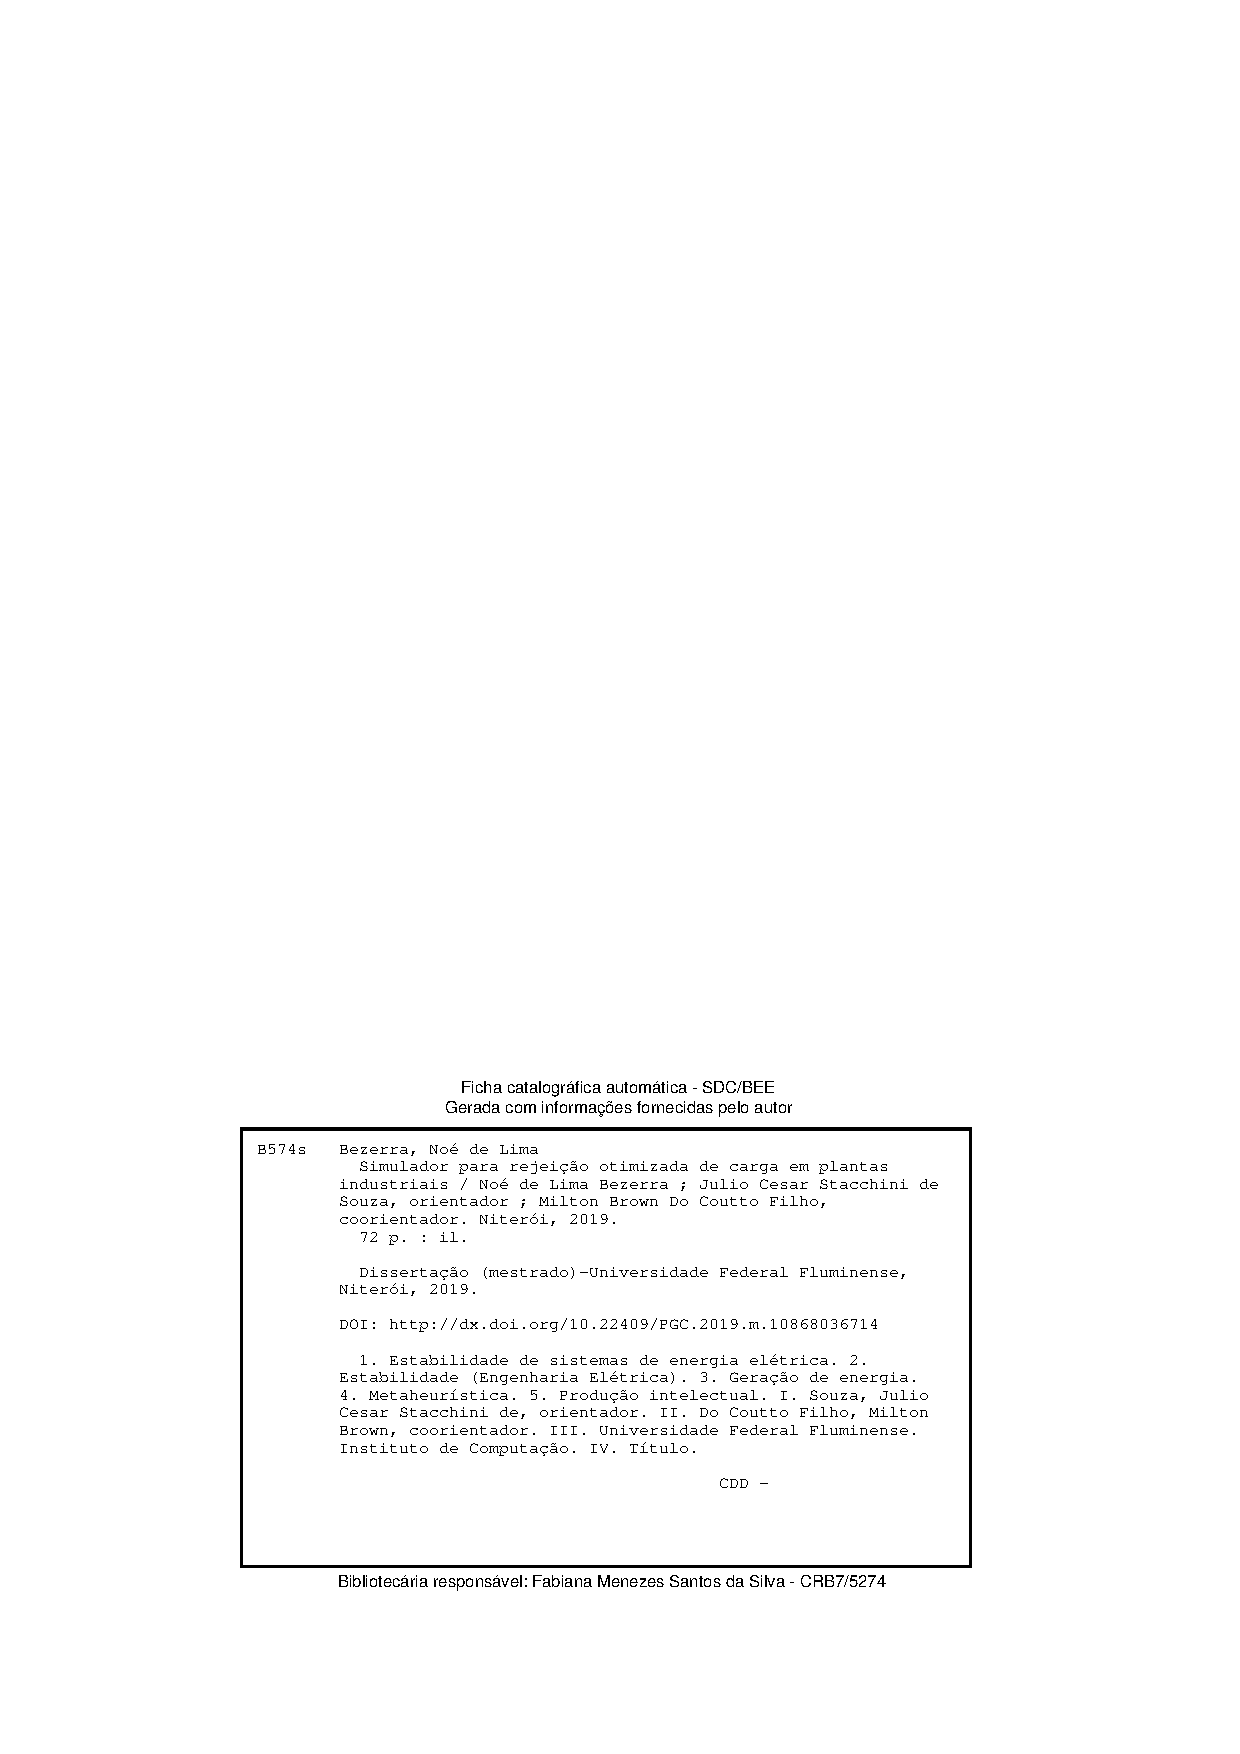
\includepdf[pages=-]{ficha_catalografica.pdf}
%\cleardoublepage
%\thispagestyle{empty}

%\vspace*{120mm}

%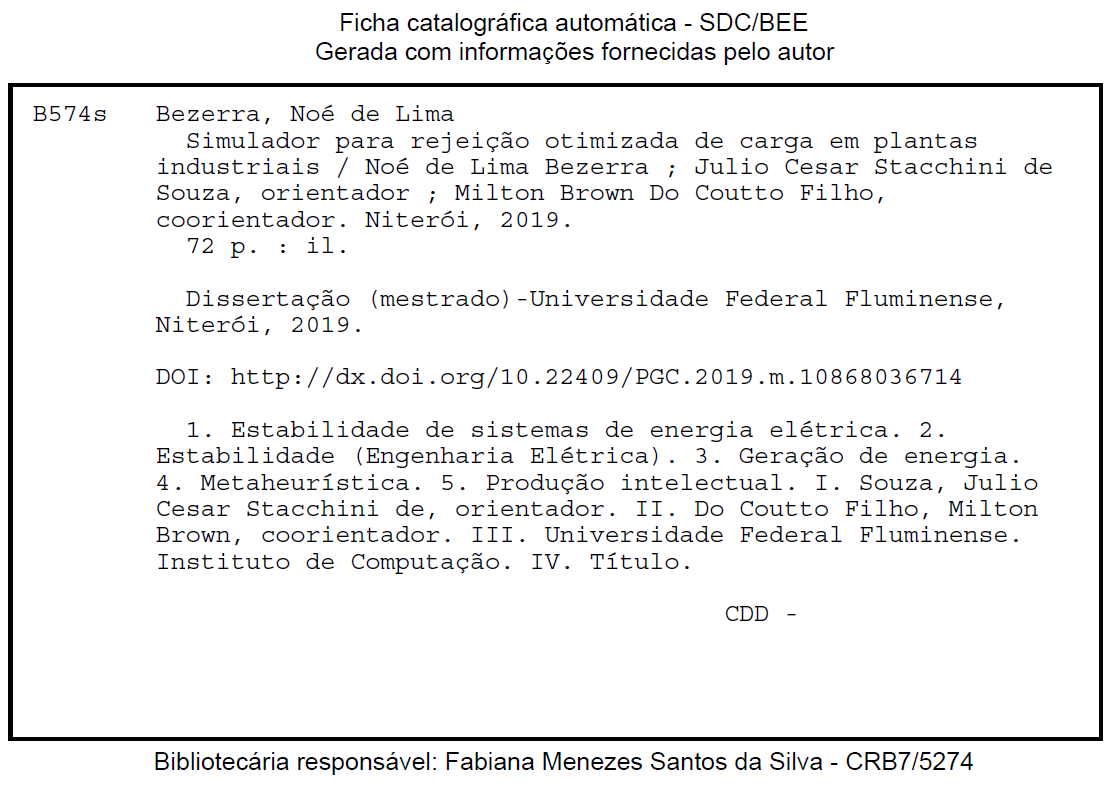
\includegraphics[width=0.9\linewidth]{figuras/ficha}


% --- -----------------------------------------------------------------
% --- Termo de aprovação. (Obrigatório)
% --- ----------------------------------------------------------------
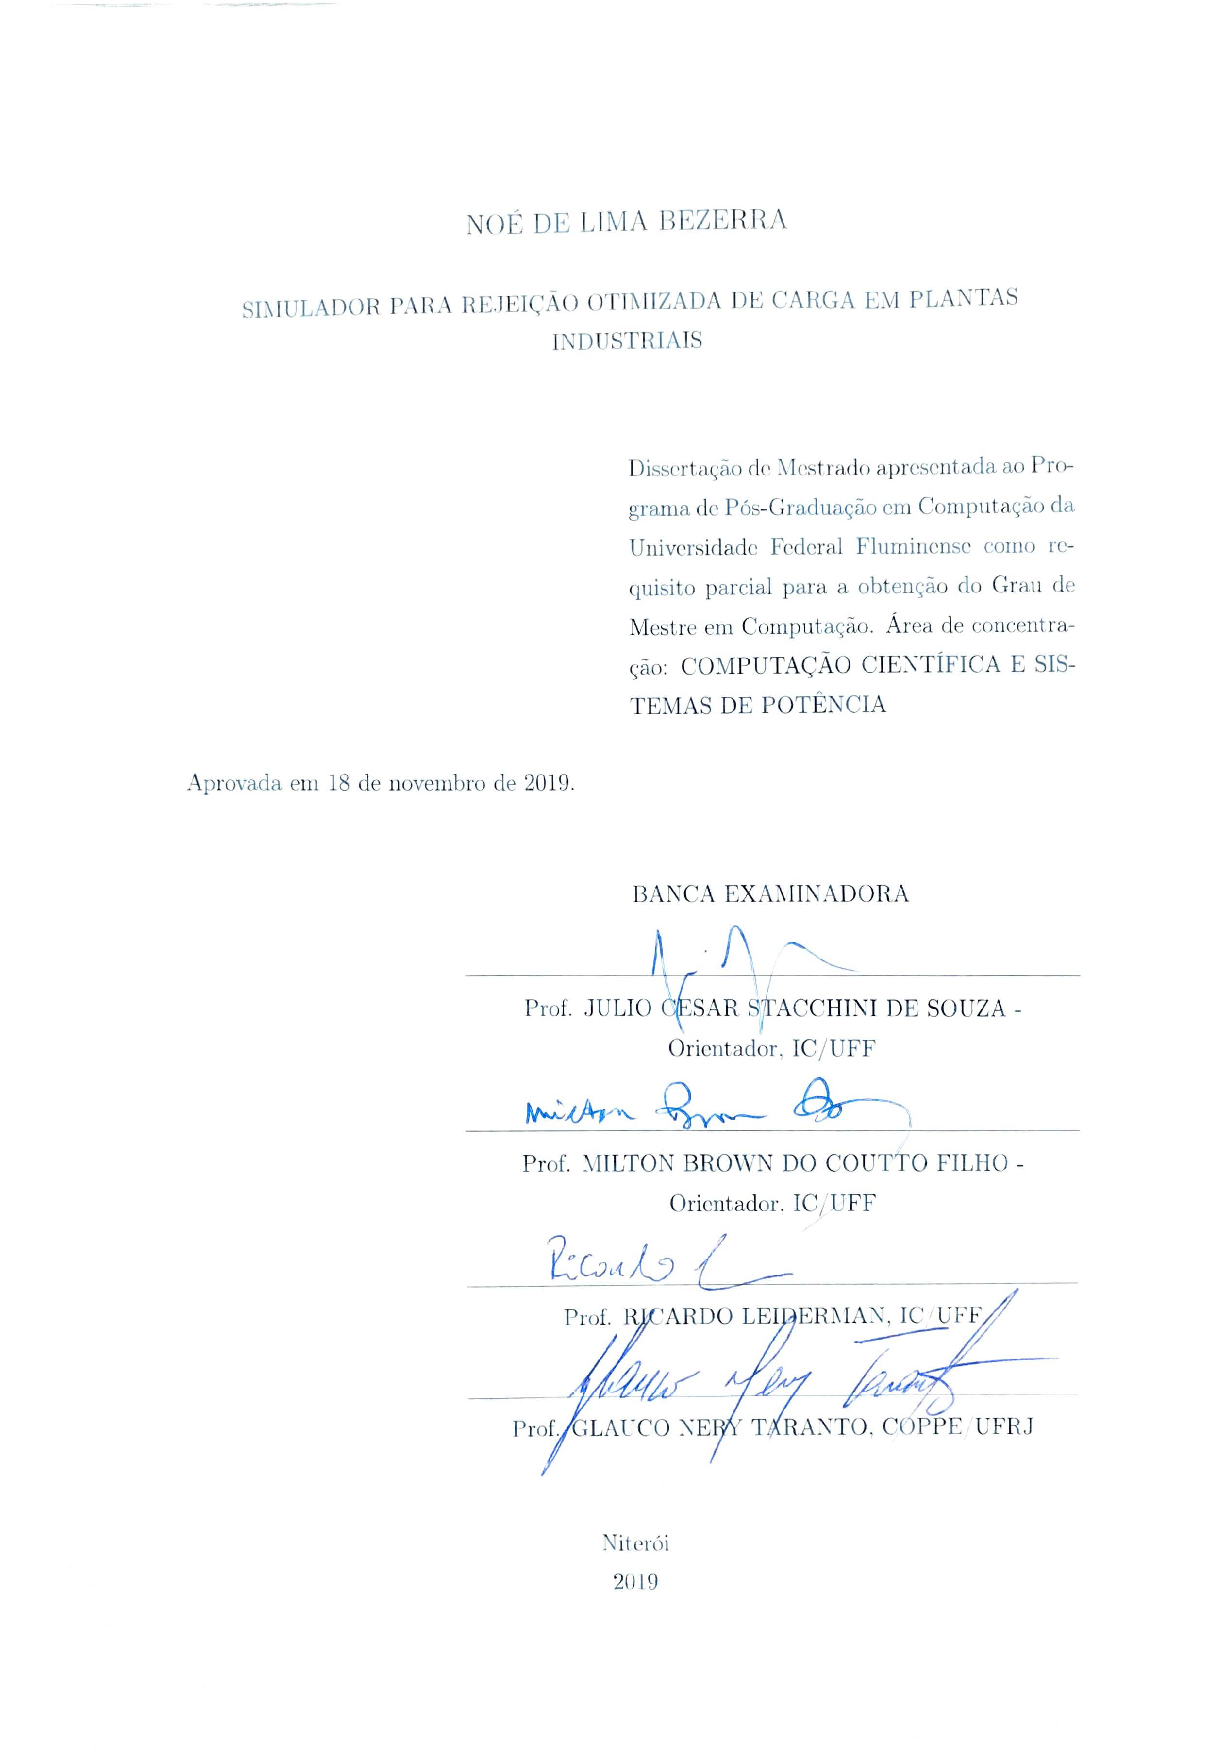
\includepdf[pages=-]{aprovacao.pdf}

% Original substituído por versão escaneada
%\cleardoublepage
%\thispagestyle{empty}

%\vspace{-60mm}

%\begin{center}
%   {\large NO{\'E} DE LIMA BEZERRA}\\
%   \vspace{7mm}

%   SIMULADOR PARA REJEI{\c C}{\~A}O OTIMIZADA DE CARGA EM PLANTAS INDUSTRIAIS\\
%  \vspace{10mm}
%\end{center}

%\noindent
%\begin{flushright}
%\begin{minipage}[t]{8cm}

%Disserta{\c c}{\~a}o de Mestrado apresentada ao Programa de P{\'o}s-Gradua{\c c}{\~a}o em Computa{\c c}{\~a}o da Universidade Federal Fluminense como requisito parcial para a obten{\c c}{\~a}o do \mbox{Grau} de Mestre em Computa{\c c}{\~a}o. {\'A}rea de concentra{\c c}{\~a}o: COMPUTA{\c C}{\~A}O CIENT{\'I}FICA E SISTEMAS DE POT{\^E}NCIA %preencha com a sua area de concentracao

%\end{minipage}
%\end{flushright}
%\vspace{5mm}
%\noindent
%Aprovada em 18 de novembro de 2019.
%\begin{flushright}
%  \parbox{11cm}
%  {
%  \begin{center}
%  BANCA EXAMINADORA \\
%  \vspace{6mm}
%  \rule{11cm}{.1mm} \\
%    Prof. JULIO CESAR STACCHINI DE SOUZA - Orientador, IC/UFF \\
%    \vspace{6mm}
%  \rule{11cm}{.1mm} \\
%    Prof. MILTON BROWN DO COUTTO FILHO - Orientador, IC/UFF \\
%    \vspace{6mm}
%  \rule{11cm}{.1mm} \\
%    Prof. RICARDO LEIDERMAN, IC/UFF \\
%  \vspace{6mm}
%  \rule{11cm}{.1mm} \\
%    Prof. GLAUCO NERY TARANTO, COPPE/UFRJ \\
%    \vspace{6mm}
%  \end{center}
%  }
%\end{flushright}
%\begin{center}
  %\vspace{2mm}
%  Niter{\'o}i \\
  %\vspace{6mm}
%  2019

%\end{center}

% --- -----------------------------------------------------------------
% --- Dedicatória.(Opcional)
% --- -----------------------------------------------------------------
\cleardoublepage
\thispagestyle{empty}
\vspace*{200mm}

\begin{flushright}
{\em 
Aos meus professores, que t{\~a}o generosamente colaboram com a continuidade e amplia{\c c}{\~a}o do conhecimento.
}
\end{flushright}
\newpage


% --- -----------------------------------------------------------------
% --- Agradecimentos.(Opcional)
% --- -----------------------------------------------------------------
\pretextualchapter{Agradecimentos}
\hspace{5mm}
{\`A} minha fam{\'\i}lia, em especial {\`a} minha esposa Camila Borduam, pelo apoio e compreens{\~a}o quanto {\`a}s noites de sono suprimidas em dedica{\c c}{\~a}o aos estudos.

Aos meus professores que, de forma generosa e altru{\'\i}sta, compartilharam comigo uma parcela de conhecimento e experi{\^e}ncia.

Aos meus orientadores, professores Milton Brown e Julio Stacchini, que pacientemente me guiaram e inflaram {\^a}nimo quando necess{\'a}rio.

Ao professor Luiz Satoru Ochi que, al{\'e}m de mostrar-se um grande amigo, providenciou todos os recursos que me foram necess{\'a}rios, bem como ensinou tudo o que aprendi sobre metaheur{\'\i}stica, grande pilar neste trabalho.

Aos meus colegas de trabalho, que colaboraram na forma{\c c}{\~a}o da minha experi{\^e}ncia profissional, bem como tornaram vi{\'a}vel a concilia{\c c}{\~a}o dos estudos com o trabalho.

Ao grande amigo que a vida me presenteou e tanto me salvou na elabora{\c c}{\~a}o desta Disserta{\c c}{\~a}o, Joubert Gon{\c c}alves.

% --- -----------------------------------------------------------------
% --- Resumo em português.(Obrigatório)
% --- -----------------------------------------------------------------
\begin{resumo}

Plantas industriais que disp{\~o}em de gera{\c c}{\~a}o pr{\'o}pria de energia el{\'e}trica podem enfrentar diversos problemas ao perder uma unidade geradora, at{\'e} mesmo aqueles da perda total do sistema el{\'e}trico. Objetivando minimizar os preju{\'\i}zos decorrentes de um completo desligamento da planta, usualmente, um sistema de rejei{\c c}{\~a}o de cargas entra em a{\c c}{\~a}o, desligando cargas selecionadas de modo a evitar a queda do restante do sistema. Este trabalho apresenta uma metodologia que busca selecionar de forma otimizada as cargas a serem desligadas, de forma a minimizar o impacto total deste desligamento. A metodologia utilizada combina um modelo matem{\'a}tico para a avalia{\c c}{\~a}o de cada solu{\c c}{\~a}o candidata e um m{\'e}todo heur{\'\i}stico de busca computacional para resolver o problema da minimiza{\c c}{\~a}o do custo operacional da planta ap{\'o}s a ocorr{\^e}ncia de um evento. Neste trabalho foi desenvolvido um simulador computacional no qual podem ser representadas as condi{\c c}{\~o}es de opera{\c c}{\~a}o da planta, a ocorr{\^e}ncia de eventos, sendo tamb{\'e}m fornecida a solu{\c c}{\~a}o otimizada para o descarte de cargas de acordo com a proposta. Tal simulador pode ser utilizado como ferramenta de suporte {\`a} tomada de decis{\~a}o, sendo tamb{\'e}m um primeiro passo na dire{\c c}{\~a}o da automa{\c c}{\~a}o das decis{\~o}es sobre rejei{\c c}{\~a}o de carga em plantas industriais. Diversos testes foram realizados para fins de valida{\c c}{\~a}o da metodologia proposta e utiliza{\c c}{\~a}o do simulador computacional desenvolvido, tendo sido caracterizados diferentes eventos em uma planta industrial adaptada a partir de um caso real. Os resultados obtidos mostram a utilidade do simulador computacional constru{\'\i}do e a efetividade da metodologia proposta na obten{\c c}{\~a}o de uma solu{\c c}{\~a}o otimizada para o problema.

{\hspace{-8mm} \bf{Palavras-chave}}: Rejei{\c c}{\~a}o de carga; descarte de carga; meta-heur{\'\i}stica; intelig{\^e}ncia computacional.

\end{resumo}

% --- -----------------------------------------------------------------
% --- Resumo em língua estrangeira.(Obrigatório)
% --- -----------------------------------------------------------------
\begin{abstract}

Industrial plants that have their own power generation can face several problems when losing a generating unit, even the critical scenario of a total loss of the electrical system. In order to minimize damages resulting from a complete shutdown of the plant, a load shedding system usually takes place, shutting down selected loads to prevent the system collapse. This Dissertation presents a methodology that seeks to optimize the process of selecting the loads to be shed, minimizing the total impact of this shutdown. The methodology proposed combines a mathematical model for the evaluation of each candidate solution with a heuristic computational search method to solve the problem of minimizing the operational cost of the plant after the occurrence of an event. A computer simulator is developed, in which the plant operating conditions are represented, as well as the occurrence of events involving the plant components. It also provides the optimized solution for the load shedding after the application of the proposed methodology. Such a simulator can be used as a decision support tool, being a first step towards the automation of decisions regarding the load rejection in industrial plants. Several tests were performed for the validation of the proposed methodology and the use of the developed computer simulator, under different operating conditions in an industrial plant adapted from a real case. The results show the usefulness of the simulator and the effectiveness of the proposed methodology in obtaining an optimized solution to the problem.

{\hspace{-8mm} \bf{Keywords}}: Load rejection; load shedding; metaheuristic; computational intelligence.

\end{abstract}

% --- -----------------------------------------------------------------
% --- Lista de figuras.(Opcional)
% --- -----------------------------------------------------------------
\cleardoublepage
\listoffigures


% --- -----------------------------------------------------------------
% --- Lista de tabelas.(Opcional)
% --- -----------------------------------------------------------------
\cleardoublepage
\label{pag:last_page_introduction}
\listoftables
\cleardoublepage

% --- -----------------------------------------------------------------
% --- Lista de abreviatura.(Opcional)
%Elemento opcional, que consiste na relação alfabética das abreviaturas e siglas utilizadas no texto, seguidas das %palavras ou expressões correspondentes grafadas por extenso. Recomenda-se a elaboração de lista própria para cada %tipo (ABNT, 2005).
% --- ----------------------------------------------------------------
\cleardoublepage
\pretextualchapter{Lista de Abreviaturas e Siglas}
\begin{tabular}{lcl}
LSS & : & \textit{Load Shedding Schedule}, Tabela de Rejei{\c c}{\~a}o de Cargas;\\
$pu$ & : & Sistema ``\textit{per unit}'', grandeza dividida por um valor de refer{\^e}ncia;\\
UFLS & : & \textit{Under Frequence Load Shedding}, Rejei{\c c}{\~a}o de Cargas por Sub-Frequ{\^e}ncia;\\
UVLS & : & \textit{Under Voltage Load Shedding}, Rejei{\c c}{\~a}o de Cargas por Sub-Tens{\~a}o;\\
ILS & : & \textit{Intelligent Load Shedding}, Rejei{\c c}{\~a}o Inteligente de Cargas;\\
ANN & : & \textit{Artificial Neural Network}, Redes Neurais Artificiais; \\
ERAC & : & Esquema Regional de Al{\'\i}vio de Carga por Sub-Frequ{\^e}ncia \\
VND & : & \textit{Variable Neighborhood Descent}, Varia{\c c}{\~a}o Descendente de Vizinhan{\c c}a; \\
GUI & : & \textit{Graphical User Interface}, Interface Gr{\'a}fica de Usu{\'a}rio; \\
API & : & \textit{Application Programming Interface}, Interface de Programa{\c c}{\~a}o; \\
CCM & : & Centro de Controle de Motor. \\
\end{tabular}

% --- -----------------------------------------------------------------
% --- Sumario.(Obrigatorio)
% --- -----------------------------------------------------------------
\pagestyle{ruledheader}
\tableofcontents


